\section{1174042 Faisal Najib Abdullah}

\subsection{Teori}
\begin{enumerate}
\item Jelaskan Apa Itu binari calssification dilengkapi ilustrasi gambar sendiri.\par
Binary Classification atau biominal adalah tugas mengklasifikasikan unsur usur dari himpunan yang diberikan kedalam kedua kelompok berdasarkan aturan klasifikasi yang telah ditetapkan. binari clasification juga dapat diartikan sebagai pembagi yang hanya memberikan dua pilihan contohnya benar dan salah atau klasifikasi tongkat panjang atau pendek. penjelasan lebih singkatnya binari classification merupakan kegiatam mengkelasifikasikan yang hanya memberikan dua class.
\begin{figure}[ht]
\centering
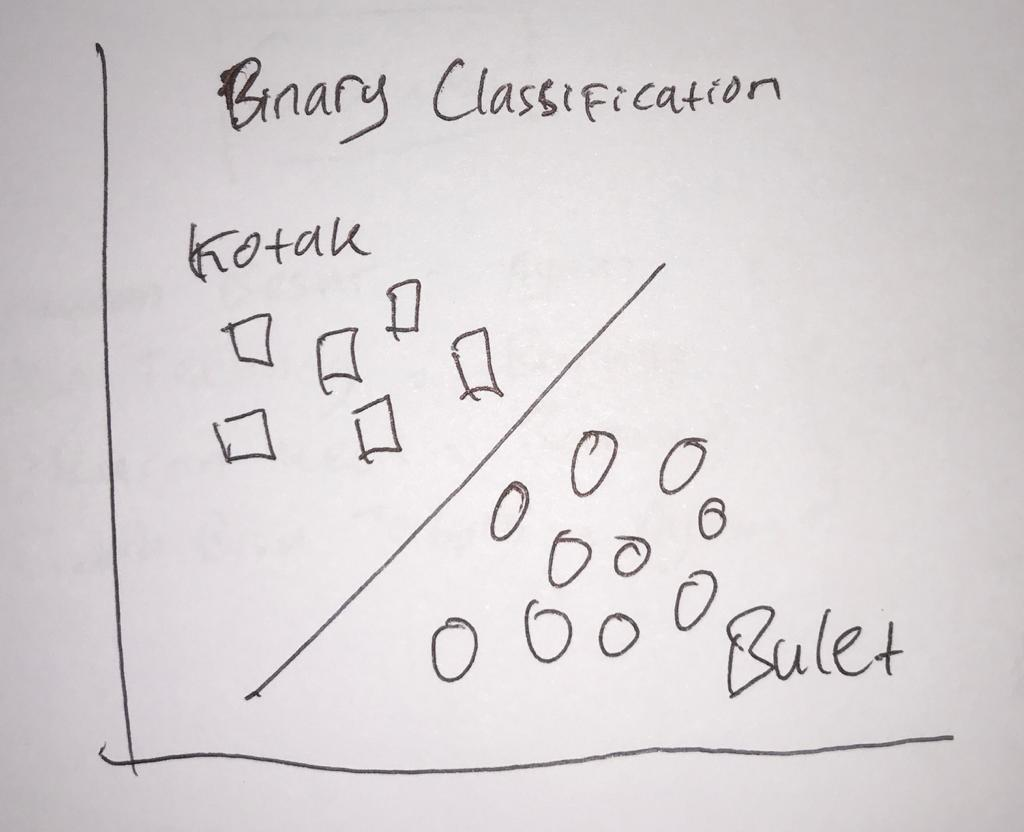
\includegraphics[scale=0.2]{figures/1174042/chapter2/1,1.jpeg}
\caption{contoh binari calssification}
\label{contoh}
\end{figure}


\item Jelaskan Apaitu supervised learning , unsupervised learning dan clusterring dengan ilustrasi gambar sendiri.\par
supervised learning adalah cara untuk mengklasifikasikan suatu objek atau data yang telah di tentukan kelas kelasnya contoh pada sayuran tumbuhan wortel termasuk yang mengandung vitamin A berarti tumbuhan wortel telah di kategorikan kedalam sayuran yang mengandung vitamin A. sedangkan kangkung mengandung zat besi yang berarti tumbuhan kangkung telah di kategorikan kedalam sayuran yang mengandung zat besi untuk lebih jelasnya dapat dilihat pada gambar.\par
\begin{figure}[ht]
\centering
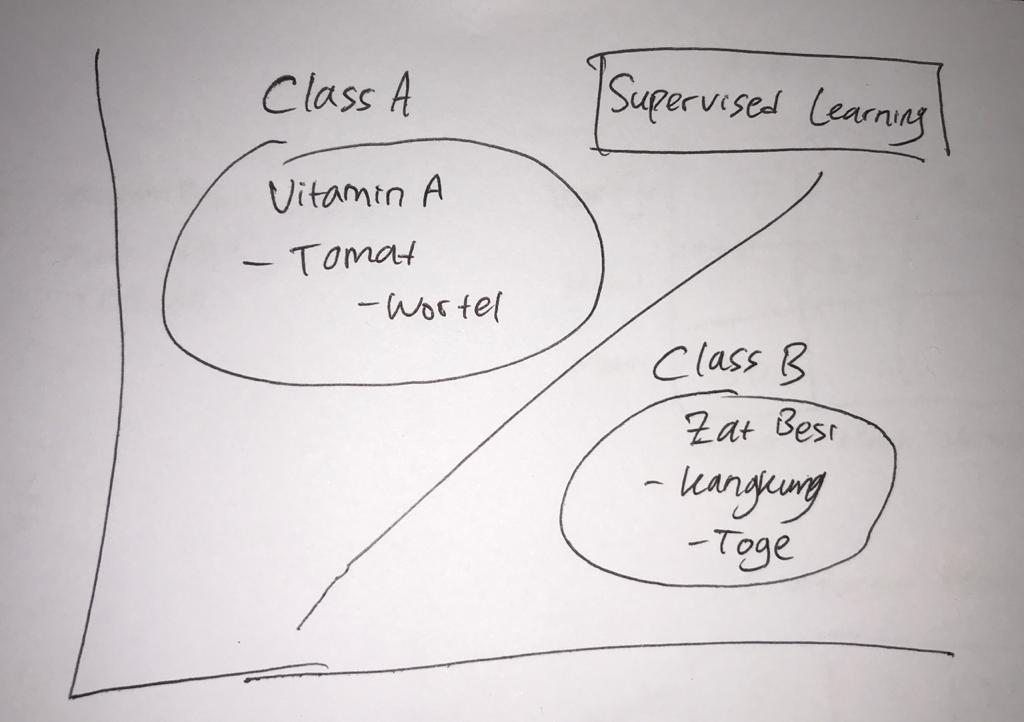
\includegraphics[scale=0.2]{figures/1174042/chapter2/1,2.jpeg}
\caption{contoh supervised learning}
\label{contoh}
\end{figure}

unsupervised learning merupakan cara untuk mengklasifikasi tanpa adanya kelas untuk menentukan jenisnya contoh sayuran berarti semua objek yang memiliki ciri ciri sayuran di kategorikan kedalam sayuran untuk lebih jelasnya dapat dilihat pada gambar.\par
\begin{figure}[ht]
\centering
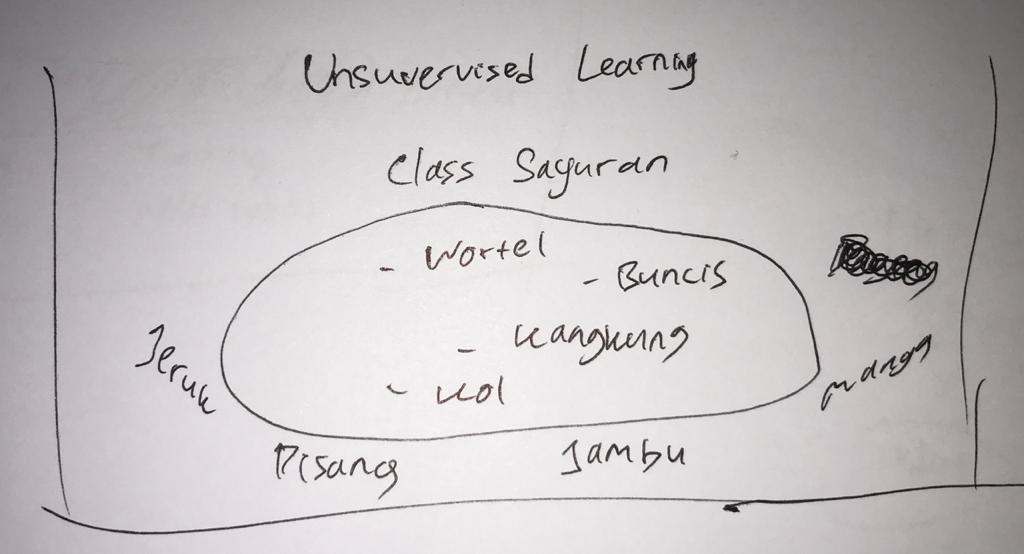
\includegraphics[scale=0.2]{figures/1174042/chapter2/1,3.jpeg}
\caption{contoh unsupervised learning}
\label{contoh}
\end{figure}

clustering merupakan peroses mengklasifikasikan yang berdasarkan suatu parameter dalam penentuannya contoh pada berat sayuran sayuran A memiliki berat 100 gr dan sayuran B memiliki berat 120 gr yang berarti berat sayuran dibagi dua parameter yaitu lebih kecil samadengan 100 gram dan lebih besar dari gram contoh pada gambar.\par
\begin{figure}[ht]
\centering
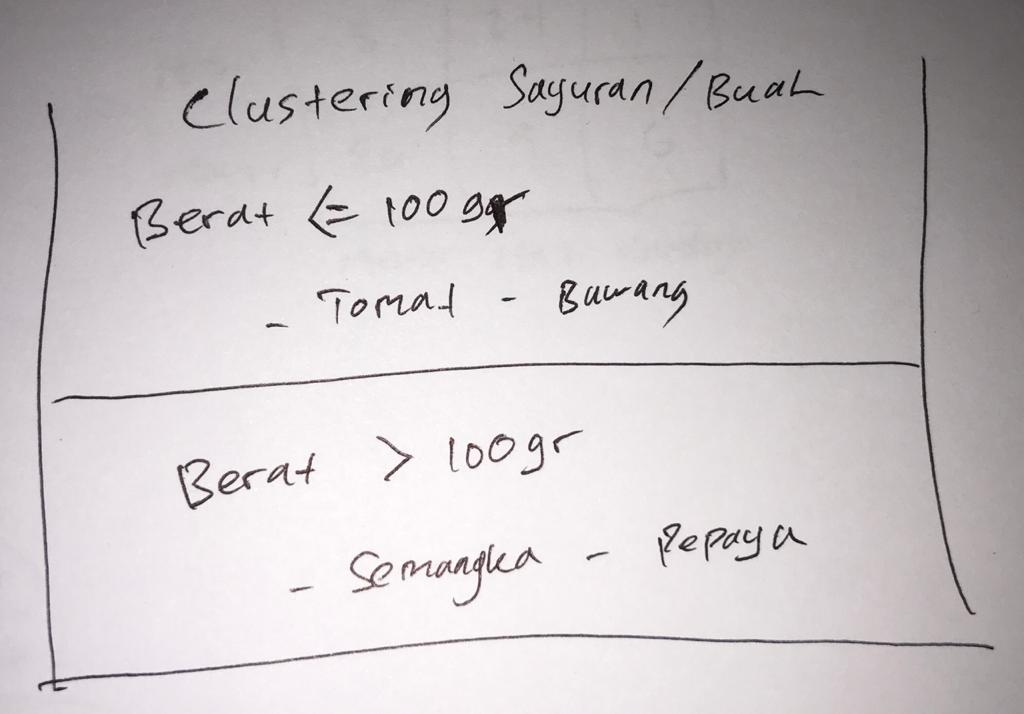
\includegraphics[scale=0.2]{figures/1174042/chapter2/1,4.jpeg}
\caption{contoh clusterring}
\label{contoh}
\end{figure}


\item Jelaskan apa itu evaluasi dan akurasi dan disertai ilustrasi contoh dengan gambar sendiri.\par
evaluasi adalah pengumpulan pengumpulan dan pengamatan dari berbagai macam bukti untuk mengukur dampak efektifitas dari suatu objek, program, atau proses berkaitan  dengan spesifikasi atau persyaratan yang telah di tetapkan sebelumnya. sedangkan akurasi itu sndiri merupakan bagian dari evaluasi yang merupakan ketepatan data terhadap suatu objek berdasarkan keriteria tertentu. kita dapat mengevaluasi seberapa baik model bekerja dengan mengukur akurasinya. ketepatan akan di definisikan sebagai presentase kasus yang di klasifikasikan dengan benar. hal ini berkaitan dengan confusion matrix pada materi selanjutnya. contoh evaluasi untuk membedakan burung dengan ayam terdapat parameter yaitu ukuran badan dan fungsi sayap pada hewan tersebut. lebih jelanya pada gambar berikut:
\begin{figure}[ht]
\centering
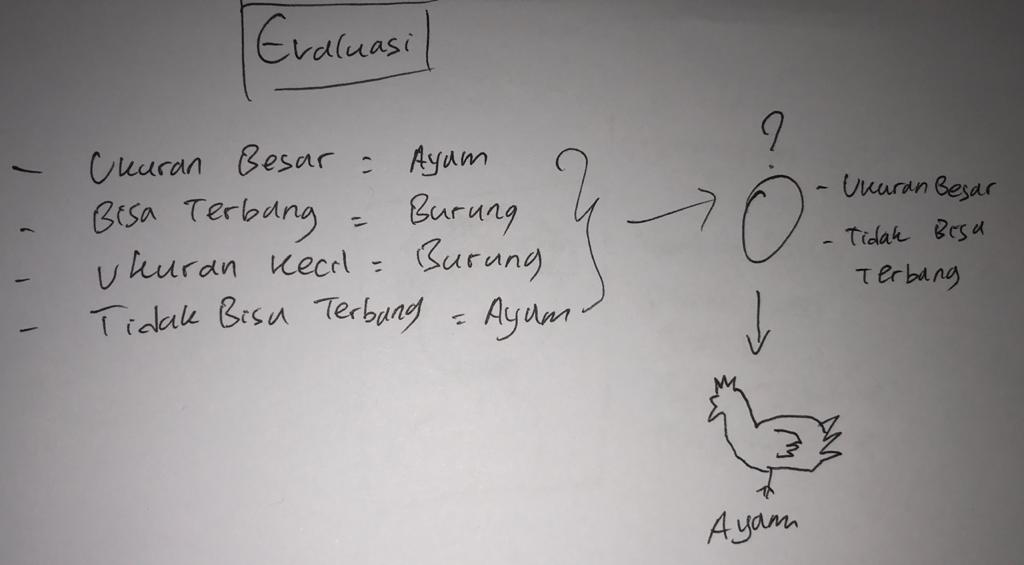
\includegraphics[scale=0.2]{figures/1174042/chapter2/1,5.jpeg}
\caption{contoh evaluasi dan akurasi}
\label{contoh}
\end{figure}


\item Jelaskan bagaimana cara membuat Confusion Matrix, Buat confusion matrix sendiri.\par
Dalam pembuatan confusion matrix tentukan parameter atau objek yang akan di evaluasi contoh bunga melati , bunga mawar, dan bunga kenangan buat tabel dengan baris dan kolom berjumlah tiga kemudian tentukan nilai miring pada setiap kolom tersebut disini saya memberi nilai 30 dengan ketentuan setiap baris harus berisi nilai 30 nilai tersebut jika terbagi ke kolom lain maka jumlahnya harus bernilai 30 jika tidak berarti data tersebut tidak akurat. untuk lebih jelanya dapat dilihat pada gambar berikut :
\begin{figure}[ht]
\centering
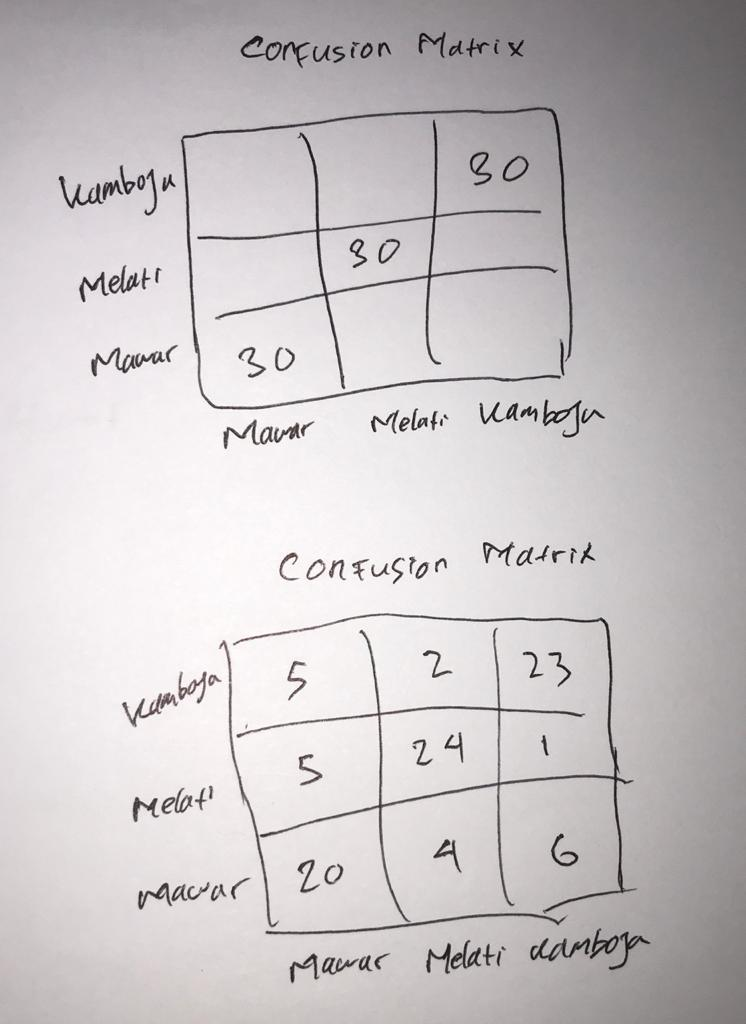
\includegraphics[scale=0.2]{figures/1174042/chapter2/1,6.jpeg}
\caption{contoh Confusion Matrix}
\label{contoh}
\end{figure}


\item Jelaskan bagaimana K-fold cross validation bekerja dengan gambar ilustrasi contoh buatan sendiri.
K-fold Cross Validation merupakan cara untuk melatih suatu mesin dimana di dalammya terdapat data set yang dibagi menjadi dua yaitu untuk data testing dan data training contoh 1000 data merupakan data set dan 200 data digunakan untuk data testing kemudian 800 datanya digunakan untuk data training dimana data training tersebut digunakan untuk menentukan nilai bobot yang dimasukan kedalam rumus regresi linier. sedangkan nilai testing akan dijadikan nili inputan untuk rumus regresi linier. contohnya dapat dilihat pada gambar berikut :
\begin{figure}[ht]
\centering
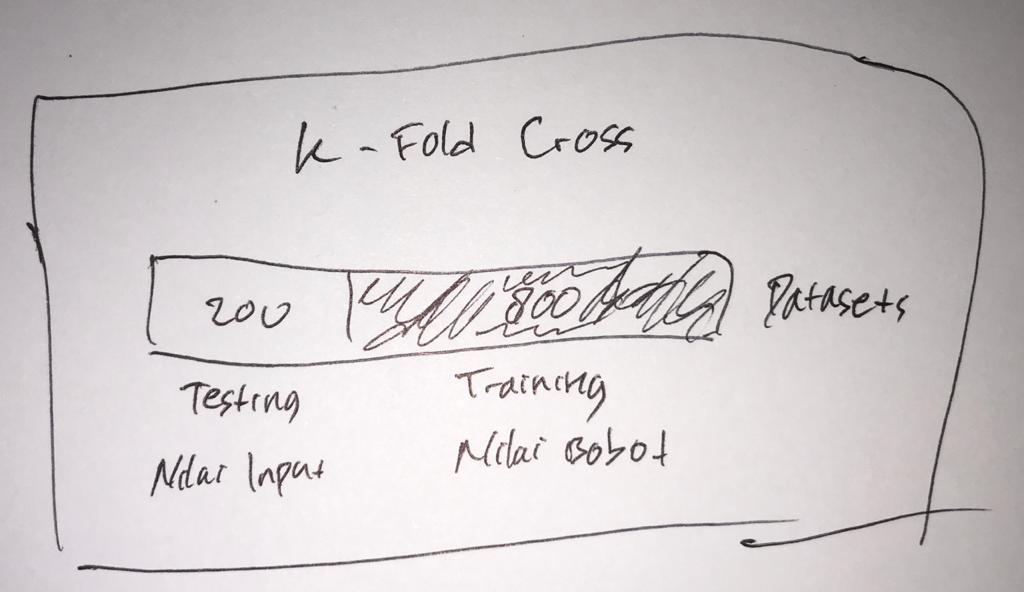
\includegraphics[scale=0.2]{figures/1174042/chapter2/1,7.jpeg}
\caption{contoh K-fold cross validation}
\label{contoh}
\end{figure}


\item Jelaskan Apa itu decision tree dengan gambar ilustrasi contoh buatan sendiri.\par
Decision tree (pohon keputusan) merupakan implementasi dari binari clasification dimana pada pohon keputusan akan terdapat root atau akar dan cabang cabangnya yang nilainya seperti if contoh pada root berisi nilai jenis kelamin, apakah perempuan pada cabang satu bernilai iya dan pada cabang dua bernilai tidak jika nilainya iya berarti jenis kelamminya perempuan dan jika tidak maka bernilai laki-laki.
agar lebih jelas dapat dilihat pada gambar decision tree berikut:
\begin{figure}[ht]
\centering
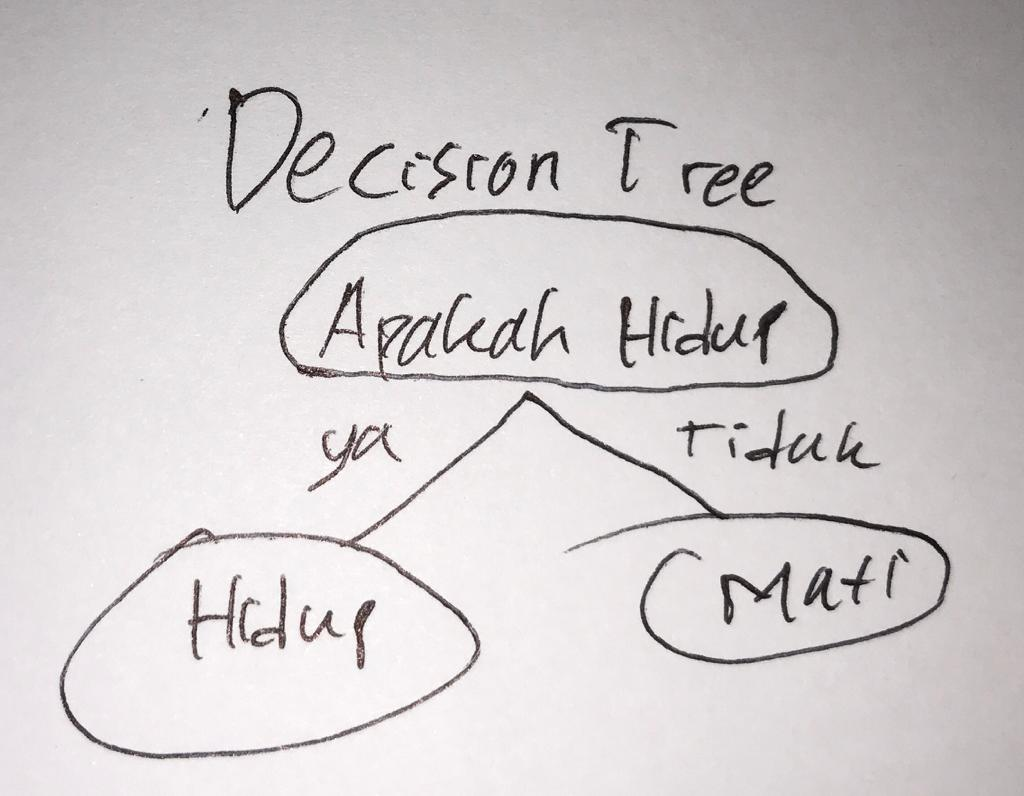
\includegraphics[scale=0.2]{figures/1174042/chapter2/1,8.jpeg}
\caption{contoh decision tree}
\label{contoh}
\end{figure}


\item jelaskan apa itu information gain dan entropi dengan gambar ilustrasi buatan sendiri.\par
informasion gain merupakan informasi atau keriteria dalam pembagian sebuah objek contoh information gain pada laki-laki yaitu berrambut lurus, mata belo, berkumis, berjenggot, dan memiliki jakun. untuk lebih jelasnya dapat dilihat pada gambar berikut :\par
\begin{figure}[ht]
\centering
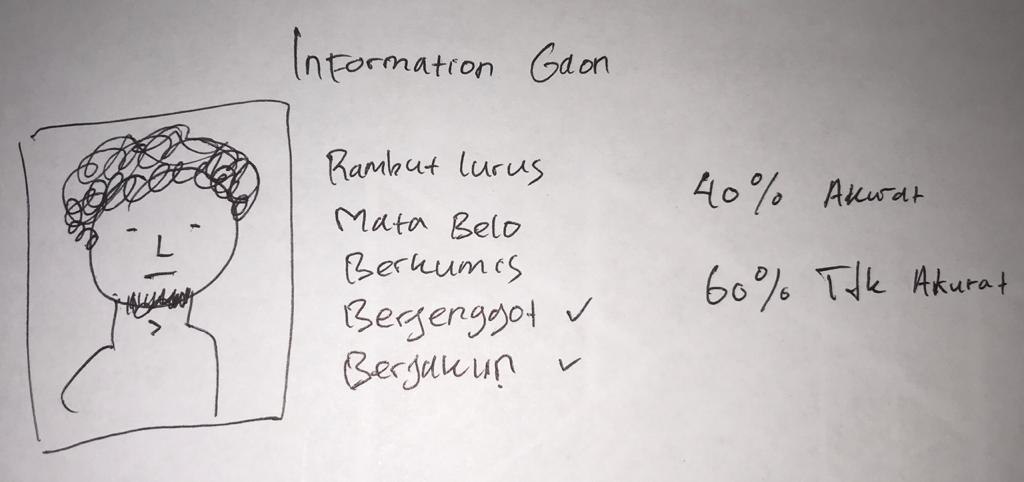
\includegraphics[scale=0.2]{figures/1174042/chapter2/1,9.jpeg}
\caption{contoh information gain}
\label{contoh}
\end{figure}
sedangkan entropi merupakan ukuran keacakan dari informasi semakin tinggi entropi maka semakin sulit dalam menentukan keputusan contoh dalam menentukan jenis kelamin semakin detail informasi maka akan semakin susah dalam menentukan keputusan.
\end{enumerate}







\subsection{Sikic-Learn}
\begin{enumerate}
\item pada surcode pertama yang dapat dilihat pada gambar pada baris pertama di tuliskan yang berarti mengimport library padas. selanjutnya pada baris ke dua codingan tersebut berisi pada code tersebut terdapat variabel muaraenim yang berisi inisialisasi padas dengan aksi untuk membaca vfile csv yang terdapat pada direktori pada komputer kemudian terdapat sep samadengan titik koma yang berarti pemisah field di dalam vile tersebut merupakan titik koma. kemudian pada bagian akhir terdapat code len (nama variabel) yang berarti akan menghotung jumlah baris pada file tersebut.
\lstinputlisting{src/1174042/chapter2/2,1.py}
\begin{figure}[ht]
\centering
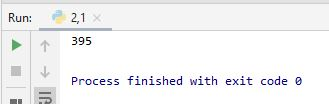
\includegraphics[scale=0.5]{figures/1174042/chapter2/2,1.JPG}
\caption{hasil}
\label{contoh}
\end{figure}

\item Pada code selanjutnya akan ditambahkan fungsi untuk lulus atau gagal yang dibuat berupa kolom kolom yang di dalammya terdapat nilai 0 dan 1 dimana 0 berarti gagal dan 1 berarti lulus. kemudian variabel pada codingan sebelumnya masih digunakan. dimana variabel muaraenim digunakan karena berisi nilai file csv kemudian dilakukan ekseskusi dengan parameter G1, G2, dan G3 dengan fungsi lambda yang berarti if bersarang atau if didalam if yang berarti nilai yang di eksekusi akan dilempar ke dalam setiap paramater sasuai dengan kriteria dan axis=1 yaitu nilai tersebut akan digunakan dari tiap baris data. sedangkan pada codingan selanjutnya variabel muaraenim di berikan aksi drop yaitu penurunan nilai pada bagian baris data. dan pada code muaraenim.head () yaitu untuk mengeksekusi codingan sebelumnya.
\lstinputlisting{src/1174042/chapter2/2,2.py}
\begin{figure}[ht]
\centering
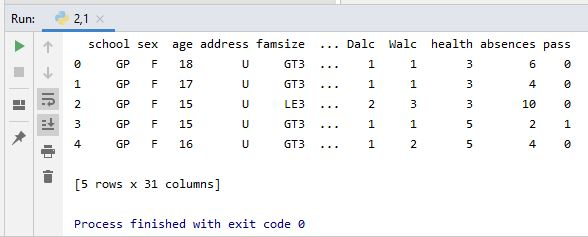
\includegraphics[scale=0.5]{figures/1174042/chapter2/2,2.JPG}
\caption{hasil}
\label{contoh}
\end{figure}

\item pada kodingan selanjutnya diguanakn untuk menambahkan nilai numerik berupa 0 dan 1 yang dirubah dari nilai tidak dan iya hal ini merupakan fungsi dari codingan get\_dummies pada baris pertama yang nilainya diambil dari variabel muaraenim yang telah di dekralasikan tadi banyaknya data numerik itu sendiri tergantung pada field dari kolom yang di camtumkan pada codingan dengan catatan field tersebut harus ada dalam data csv yang di import oleh codingan pertama tadi maka hasilnya akam merubah data dalam field tersebut menjadi 0 dan 1.
\lstinputlisting{src/1174042/chapter2/2,3.py}
\begin{figure}[ht]
\centering
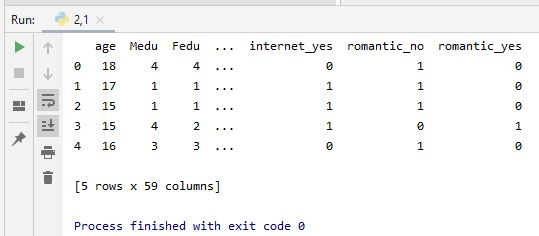
\includegraphics[scale=0.5]{figures/1174042/chapter2/2,3.JPG}
\caption{hasil}
\label{contoh}
\end{figure}

\item selanjutnya pada codingan selanjutnya yaitu menentukan data training dan data testing dari dataset dimana variabel muaraenim yang berisi data csv tadi dibuat perbandingan 500 untuk data training dan sisanya yaitu 149 digunakan untuk data testing hal ini di lakukan pada baris ke 1 sampai ke 3 pada gambar kemudian nilai tersebut di turunkan  brdasarkan baris pada data set hal itu dapat dilihat pada baris ke 4 sampai ke 9 pada gambar kemudian selanjutnya mengimport library numpy yang berguna untuk oprasi vektor dan matrix karna data diatas berupa data matrix maka library ini di gunakan.
\lstinputlisting{src/1174042/chapter2/2,4.py}
\begin{figure}[ht]
\centering
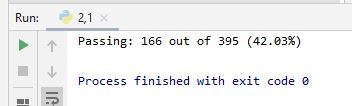
\includegraphics[scale=0.5]{figures/1174042/chapter2/2,4.JPG}
\caption{hasil}
\label{contoh}
\end{figure}

\item selanjutnya yaitu membuat pohon keputusan pada baris pertama yairu memasukan librari tree kemudian pada baris kedua dibuat variabel palembang dengan nilai DecisionTreeClasifier yang merupakan paket atau fungsi dari scikit-learn yang merupakan class yang mampu melakukan multi class. sedangkan max\_depth=5 merupakan untuk penyesuaian data terhadap pohon keputusan itu sndiri.
\lstinputlisting{src/1174042/chapter2/2,5.py}
\begin{figure}[ht]
\centering
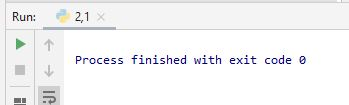
\includegraphics[scale=0.5]{figures/1174042/chapter2/2,5.JPG}
\caption{hasil}
\label{contoh}
\end{figure}

\item selanjutnya yaitu pembuatan gambar dari pohon keputusan yang tadi di buta pada codingan sebelumnya pada baris pertama codingan ya itu mengimport library graphviz kemudian pada baris ke dua yaitu pemberian nilai pada variabel baru dot data nilainy diambil dari pembuatan puhon keputusan tadi kemudian di tentukannya nilai benar dan salah dari codingan tersebut setelah itu dibuatlah sebuah variabel untuk menampung hasil eksekusi tersebut kemudian variabel tersebut di running.
\lstinputlisting{src/1174042/chapter2/2,6.py}
\begin{figure}[ht]
\centering
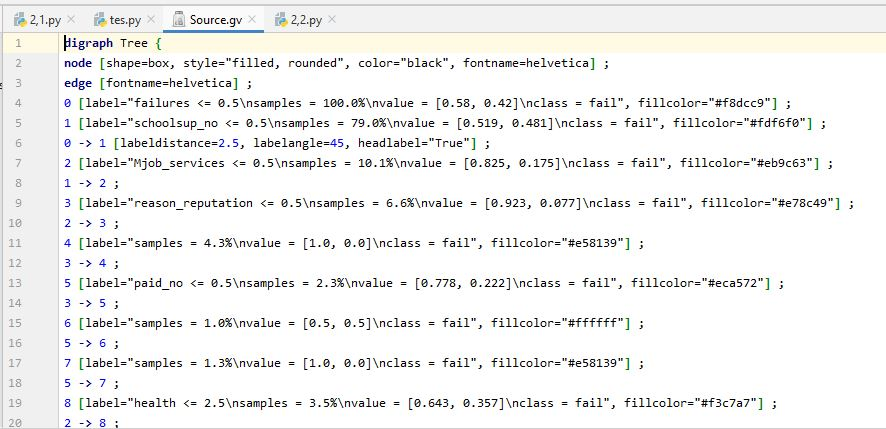
\includegraphics[scale=0.5]{figures/1174042/chapter2/2,6.JPG}
\caption{hasil}
\label{contoh}
\end{figure}

\item selanjutnya pembuatasn method untuk menyimpan data pohon dengan menarik data langsung dari pohon keputusan.
\lstinputlisting{src/1174042/chapter2/2,7.py}
\begin{figure}[ht]
\centering
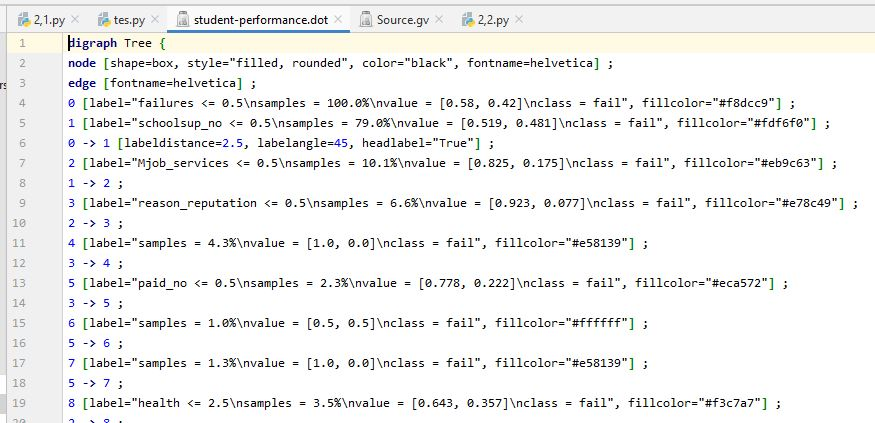
\includegraphics[scale=0.5]{figures/1174042/chapter2/2,7.JPG}
\caption{hasil}
\label{contoh}
\end{figure}

\item selanjutnya pada codingan berikut yaitu digunakan untuk mencetak nilai score rata-rata dari ketepatan data yang telah di olah.
\lstinputlisting{src/1174042/chapter2/2,8.py}

\item selanjutnya yaitu digunakan untuk memeriksa akurasi dari ketepatan hasil pengolahan data tersebut maka akan didapat nilai rata-rata 60 persen dari hasil pengolahan data tersebut, pada codingan tersebut pada baris ke satu melakukan import library dari sklern kemudian pada baris selanjutnya mengisi nilai skor dengan nilai pada variabel palembang setelah hal tersebut dilakukan kemudian data tersebut di eksekusi.
\lstinputlisting{src/1174042/chapter2/2,9.py}
\begin{figure}[ht]
\centering
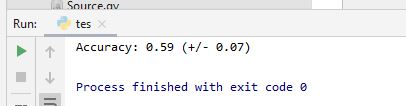
\includegraphics[scale=0.5]{figures/1174042/chapter2/2,9.JPG}
\caption{hasil}
\label{contoh}
\end{figure}

\item membuat rank akurasi dari 1 sampai 100 untuk melihat akurasi data apakah datatersebut terdapat di rata rata 60 persen atau tidak dengan cara membuat lagi variabel baru dengan nilai tree diadalammya jadi hampir mirip seperti membuat pohon keputusan namun ini langsung dalam bentuk rata rata akurasi yanlebih spesifik.
\lstinputlisting{src/1174042/chapter2/2,10.py}
\begin{figure}[ht]
\centering
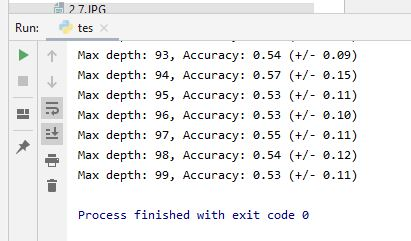
\includegraphics[scale=0.5]{figures/1174042/chapter2/2,10.JPG}
\caption{hasil}
\label{contoh}
\end{figure}

\item untuk selanjutnya yaitu menentukan nilai untuk grafik hampirsama dengan nilia akurasi tadi pertama tentukan rank atai batasan nilai itu disini batasannya di mulai dari 1 sampai 20 dengan menggunakan nilai tree tadi maka hasilnya dapat ditentuka kemudian buat variabel i untuk penomoran tiap record yang keluar atau recod hadil dari eksekusi tree tersebut.
\lstinputlisting{src/1174042/chapter2/2,11.py}
\begin{figure}[ht]
\centering
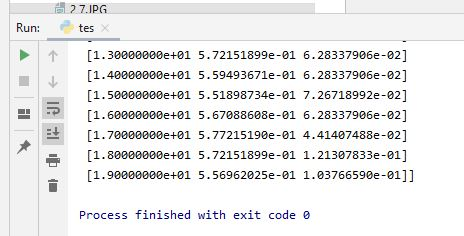
\includegraphics[scale=0.5]{figures/1174042/chapter2/2,11.JPG}
\caption{hasil}
\label{contoh}
\end{figure}

\item terakhir yaitu pembuatan grafik untuk pembuatan grafik diambil data dari codingan sebelumnya yang 20 record tadi dengan cara mengimport libray matplotlib.pyplot yang di inisialisasi menjadi bakwankemudian inisialisasi tersebut di eksekusi.
\lstinputlisting{src/1174042/chapter2/2,12.py}
\begin{figure}[ht]
\centering
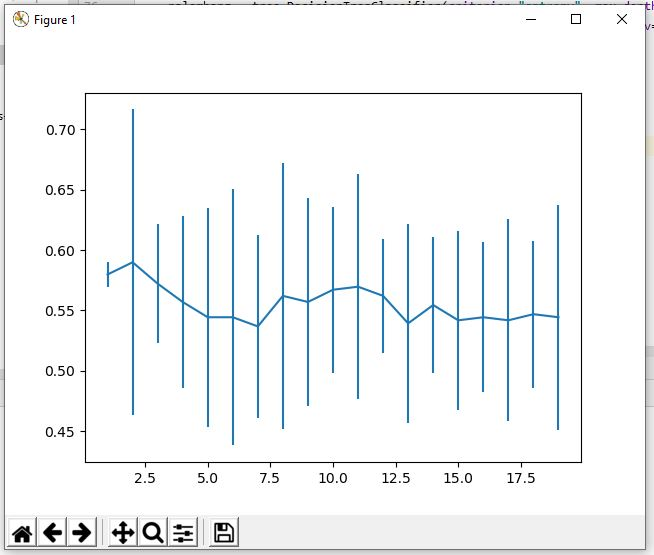
\includegraphics[scale=0.5]{figures/1174042/chapter2/2,12.JPG}
\caption{hasil}
\label{contoh}
\end{figure}
\end{enumerate}

\subsection{Penanganan Error}
\begin{enumerate}
\item skrinsut error
\begin{figure}[ht]
\centering
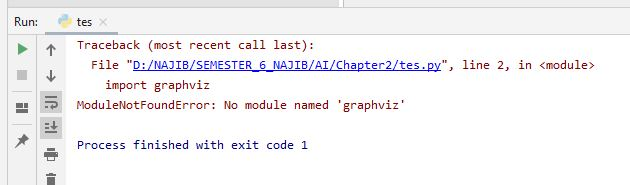
\includegraphics[scale=0.5]{figures/1174042/chapter2/error.JPG}
\caption{Error}
\label{contoh}
\end{figure}

\item kode error dan jenis errornya .
\begin{verbatim}
import graphviz
dot_data = tree.export_graphviz(palembang, out_file=None, label="all", impurity=False, proportion=True,
                                feature_names=list(muaraenim_train_att), class_names=["fail", "pass"], 
                                filled=True, rounded=True)
graph = graphviz.Source(dot_data)
graph
\end{verbatim}

pada codingan tersebut error karena graphiznya belu di istall 

\item Solusi pemecahan masalah \par
buka CMD komputer anda run as administrator koemudian masukan perintah conda install graphviz.
\end{enumerate}


\subsection{Plagiat}
\begin{figure}[ht]
\centering
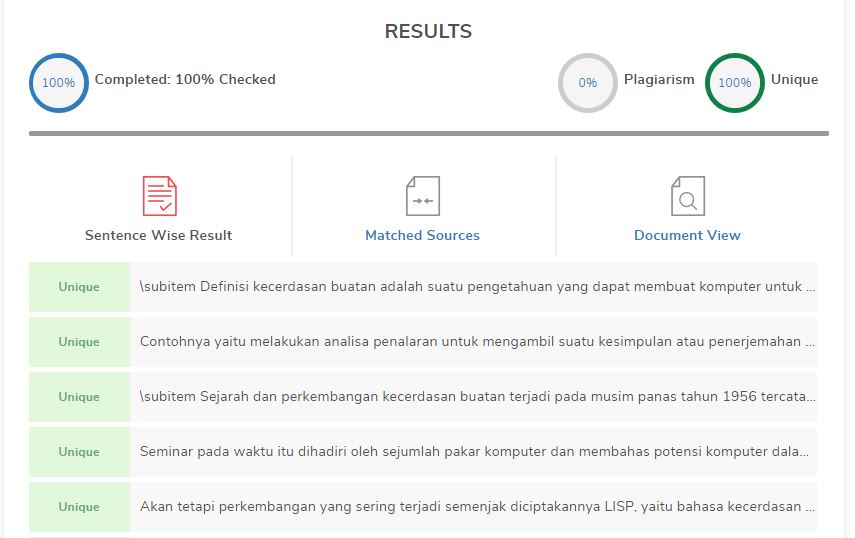
\includegraphics[scale=0.5]{figures/1174042/chapter2/plagiat.jpg}
\caption{Error}
\label{contoh}
\end{figure}
